\documentclass[11pt]{article}

\usepackage[utf8]{inputenc}
\usepackage[T1]{fontenc}
\usepackage[margin=1in]{geometry}
\usepackage{algorithm}
\usepackage{algpseudocode}
\usepackage{tikz}
\usepackage{amsmath, amssymb}
\usepackage{float}
\usetikzlibrary{trees}

\bibliographystyle{plain}


\title{TODO Add a name}
\author{Kevin Chen}
\date{\today}

\begin{document}

\maketitle

\section{Introduction}

TODO insert introduction

\section{Symbolic Execution}

Symbolic execution is a way of executing a program abstractly, such that on abstract execution covers multiple possible inputs of the program that share a particular execution path through the code \cite{aldrich2018symbolic}. Each input of symbolicly executed code is represented as a symbol rather than assigning it a concrete value. When the value is referenced such as for an if statement, the execution path branches, where one path the symbolic value is evaluated as true while the other path the symboilic value is evaluated as false.

One of the key uses for symboli execution is in testing. Most unit tests, require the programmer to hardcode in values to test, resulting in various unit tests to cover all branches the code can tranverse. On the other hand, a symbolic execution would execute simutaneously on a family of inputs. Consider the following example:

\begin{algorithm}
    \caption{Algorithm 1}
    \begin{algorithmic}[1]
    \Require $x, y \in \mathbb{Z}$
    \State $a \gets x + y$
    \If{$a \bmod 2 = 0$}
        \State \Return error ``$a$ is even''
    \Else
        \State \Return $a$
    \EndIf
    \end{algorithmic}
\end{algorithm}
    
With a glance, we can see that using any combination of numbers such that their sum results in an even number will result in an error. There is no way to cover all cases of failure using unit tests, as there are an infinite number of way which we can stumble onto this error.

Instead of testing with unit tests such as $x=1, y=1$, symbolic execution represents the inputs as symbols $x=x_0, y= y_0$. Whenever, the symbols are required to return a value, such as in a branch, symbolic execution splits into two executions, with each execution recording the branching condition in its execution path. Consider a symbolic execution of the algorithm above. We start with representing each input symbolicly:

\begin{figure}[H]
    \centering
    \begin{tabular}{|c|c|c|}
        \hline
        line & Path Condition & Translation \\
        \hline
        0 & true & $x\to x_0, y\to y_0$ \\
        1 & true & $x\to x_0, y\to y_0, a\to x_0+y_0$ \\
        2 & $(x_0 + y_0) \bmod 2 = 0$ & $x\to x_0, y\to y_0, a\to x_0+y_0$ \\
        2 & $\neg((x_0 + y_0) \bmod 2 = 0)$ & $x\to x_0, y\to y_0, a\to x_0+y_0$ \\
        3 & $(x_0 + y_0) \bmod 2 = 0$ & Error \\
        5 & $\neg((x_0 + y_0) \bmod 2 = 0)$ & Return $x_0 + y_0$ \\
        \hline
    \end{tabular}
    \caption{Symbolic execution trace showing path conditions and variable translations}
    \label{fig:symbolic-trace}
\end{figure}

In this example, we see that the inputs values start symbolic as symbols which has no concrete value. Following the execution, we translate every instance of $x$ with $x_0$ with the same case for $y$. Where it gets interesting is when the the execution has a branching path. In the $\textbf{if}$ statement, the value of a is required to be assigned a value, which breaks the symbolic abstraction. Instead, the symbolic execution branches into two different executions, each of which assuming a different condition to satisfy the branching statement. Below we can visualize the different execution paths the execution takes via a simple tree (see Figure~\ref{fig:execution-tree}):

\begin{figure}[H]
    \centering
    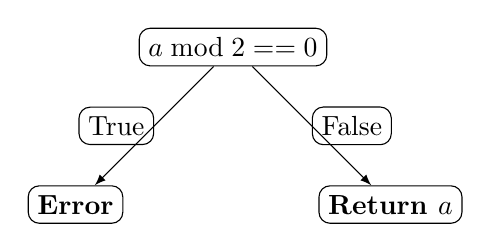
\begin{tikzpicture}[
        level distance=2cm,
        sibling distance=4cm,
        every node/.style={draw, rounded corners, align=center},
        edge from parent/.style={draw, -latex}
      ]
      
      \node {$a \bmod 2 == 0$}
          child { node {\textbf{Error}}
              edge from parent node[left] {True}
          }
          child { node {\textbf{Return $a$}}
              edge from parent node[right] {False}
          };
      
      \end{tikzpicture}
    \caption{Execution tree showing the branching paths in symbolic execution}
    \label{fig:execution-tree}
\end{figure}

In each paths, we accumulate the different path conditions until we either reach the end (return statement) or a failure (error). In this case, we find that there exists a set of inputs (when $x_0+y_0 \bmod 2 = 0$), which causes an error. Prior to running this program with symbolic execution, one can add constraints to the path. Below, an example where we start with a given constraint that $x_0+y_0=1$:

\begin{figure}[H]
    \centering
    \begin{tabular}{|c|c|c|}
        \hline
        line & Path Condition & Translation \\
        \hline
        0 & $x_0+y_0=1$ & $x\to x_0, y\to y_0$ \\
        1 & $x_0+y_0=1$ & $x\to x_0, y\to y_0, a\to x_0+y_0$ \\
        2 & $\neg((x_0 + y_0) \bmod 2 = 0)$ & $x\to x_0, y\to y_0, a\to x_0+y_0$ \\
        2 &  $x_0+y_0=1 \land (x_0 + y_0) \bmod 2 = 0$ & $x\to x_0, y\to y_0, a\to x_0+y_0$ \\
        3 & False & Error \\
        5 & $\neg((x_0 + y_0) \bmod 2 = 0)$ & Return $x_0 + y_0$ \\
        \hline
    \end{tabular}
    \caption{Modified version of execution with existing constraints}
    \label{fig:symbolic-trace-with-constraint}
\end{figure}

With the constraint, the path condition which leads to the error is contradictory. This illustrates that the path is impossible. With this constraint, we see that no path leads to any errors. In industry, programmers, can create tests with given preconditions (constraints) and run until the program terminates. Instead of throwing an error, we can use assertion statements as post-conditions. If it terminates without an error, the program is robust across all set of inputs. Otherwise, a symbolicly executed program will return a concrete set of conditions which will give an error or violate a post-condtiion.

\section{My Program}

\subsection{Execution Path}




\section{Conclusion}

\bibliography{references}

\end{document}
